\chapter{Change-point detection for concentration data}\label{chp:4}

\minitoc

\clearpage

In this Chapter, we build a change-point detection algorithm specially adapted for concentration data. We will use that algorithm to detect homogeneous temporal periods on which spatial statistical inferences will be possible. Several elements presented in Chapter \ref{chp:3} are used to build this method:  
\begin{itemize}
\item We use a parametric change-point detection, more precisely a maximum likelihood based method as described in Section \ref{chp:3:1}. The cost function $W$ is defined as the negative log likelihood of a distribution $Q$. The choice of $Q$ is motivated by the observation of the data, see Chapter \ref{chp:5} for an illustration on pesticide concentration data modeling.  
\item We use the PELT search method presented in Section \ref{chp:3:2} to obtain optimal solution to the change-point detection problem. Several penalty values $\beta$ are explored with the CROPS algorithm shown in Section \ref{chp:3:3}. The elbow method is applied when it is necessary to estimate an optimal number of change-points.   
\end{itemize}
We first describe the model integrating the censorship information in Section \ref{chp:4:1}. However, we don't known how much the censorship can affect a parametric change-point model. We provide a study of censoring effects in Section \ref{chp:4:2}. Futhermore, we need to devise an estimation procedure that is adapted to the observations of pesticide concentrations. The question sums up to detecting breaks in all dimensions of the parameters of $Q$ or not. We devise our estimation scheme in Section \ref{chp:4:3}. Finally we test our method with a change-point method adapted for censored data in Section \ref{chp:4:4}.  


\section{Generic model for censored data}\label{chp:4:1}

We present here the underlying parametric model we are using. We condider $\bm c = c_1,\dots,c_n$ that are realizations of independant random variables $C_1,\dots,C_n$. The variables $C_i$ are recorded sequentially, and the recording times are not necessarily equidistant. Thus, the indices in $Y_i$ are only indicators of the order of occurrence in the sample and not of the observation times. We suppose that there exist $K^*$ changes in the distribution of $\bm c$ happening at index $0=\tau_0^*<\tau^*_1 <... < \tau^*_k <... < \tau^*_{K^*}<\tau^*_{K^*+1}=n$. Moreover, on the k-th segment, $C_{\tau^*_{k-1}+1:\tau^*_{k}}$ follows a distribution $Q$ with parameters defined by the vector $\theta^*_k\in\Theta$ with $\Theta\subset\mathbb{R}^P$. We denote $\bm{\theta^*} = (\theta^*_k)_{k=0}^{K^*}$. More formally, we have that:  
$$c_t \sim f(.;\theta^*_k)\mathbbm{1}_{\tau^*_{k}+1\leq t \leq \tau^*_{k+1}},$$
$f$ being the density function of distribution $Q$.  


The observations are subject to censorship. We focus on left-censorship because it is adapted for modeling concentration data but similar models can be created for right censorship or a mix of both. To each $c_i$ is associated a known censoring threshold $a_i$. The resulting censored observations are defined by:  
\begin{equation}\label{chp:4:defy}
Y_i = \sup(C_i,a_i)
\end{equation}
Since the $C_i$ are independant and the $a_i$ are known deterministic values, the $Y_i$ are independant as well. The observations of $Y_i$ are denoted $y_i$. Noting $F$ the cumulative distribution function (cdf) of $Q$, we can write the cost function associted to segment $y_{u:v}$ as:  
\begin{equation}\label{chp:4:costfunc}
W(y_{u:v}) = -\sup_{\theta \in \Theta}\{\sum_{i=u}^v\log(F(y_i,\theta))\mathbbm{1}_{y_i=a_i}+\sum_{i=u}^v\log(f(y_i,\theta))\mathbbm{1}_{y_i>a_i}\}
\end{equation}
Note that if one needs to integrate right censorship into the likelihood, one should simply replace the $\sup$ in the definition \ref{chp:4:defy} by the $\inf$ of both quantities and cdf function $F$ by the survival function $S(t)=1-F(t)$. 
For a segmentation $\TT = \{\tau_1,...,\tau_K\}$, the penalised cost is given by: 
\begin{equation}\label{chp:4:pencost}
\CC(\bm y,\TT)=\sum_{i=0}^{K}  W(y_{\tau_i+1:\tau_{i+1}}) + KP\beta,
\end{equation}
where $P$ is the dimension of the parameters vector in the distribution $Q$. Gathering \ref{chp:4:costfunc} and \ref{chp:4:pencost}, this resulting estimator can be expressed as:  
\begin{equation}\label{chp:4:estim}
(\widehat{\TT},\widehat{\bm \theta}) = \arg\min_{\TT,\bm \theta} \left(- \sum_{i=0}^{\lvert \TT \rvert}  \left\{\sum_{j=\tau_i+1}^{\tau_{i+1}}\log(F(y_j,\theta))\mathbbm{1}_{y_j=a_j}+\sum_{j=\tau_i+1}^{\tau_{i+1}}\log(f(y_j,\theta))\mathbbm{1}_{y_j>a_j}\right\}+\beta KP\right)
\end{equation}

Under this configuration, we know that the estimators computed \ref{chp:4:estim} have satisfying convergence properties \citep{Lavielle1997}. Elements of proof are provided in Appendix \ref{app:chap4:1}.

\section{Censorship effects}\label{chp:4:2}

We are interested in the effects of censorship on two main aspects: 
\begin{itemize}
\item The estimation of the parameters $\bm \theta$ of $Q$ on a fixed segment. 
\item The implication it can have on the search method PELT and how to adapt it if this is the case. 
\end{itemize} 
Illustrating examples are provided in this section with $Q$ set as the exponential distribution.

\subsection{On the parameter estimation for one segment}

In general, an explicit formula for the maximum likelihood estimator (MLE) is not available in presence of censored data, leading to the use of numerical methods for its computation. The Newton-Raphson method was used on each segment to compute the MLE estimate of $\theta$. The cost functions need to be twice differentiable in $\theta$. We search for the zeros of the first derivate of the cost function in order to find a global minimum. 

Checking that the second derivative is strictly positive in presence of censored data, thus guaranteeing the unicity of the maximum likelihood estimate, can prove to be a difficult task as it is not always the case for all distribution $Q$. We provide an example of such a case in Appendix \ref{app:chap4:2} where we prove the existence of a global minimum without having the global convexity of the first derivate. This implies that a careful initialization of the Newton-Raphson method to obtain convergence. Appendix \ref{app:chap4:2} also provide experiments on the initialization of the Newton-Raphson method. 

Specifically, the case where all data in the segment $y_{u:v}$ are censored is problematic. Looking at the analytical likelihood formula, we find that the $\theta$ realising the minimum of the cost function is still unique, but tends toward infinity. In this case the cost tends to zero. We illustrate in Figure \ref{fig:onlycens} with $Q$ set as an exponential distribution. 

For a given segment $y_{u:v}$ where all observations are censored and under a censorship threshold $a$ we have that: 
\begin{equation} \label{chp:4:costex}
W(y_{u:v}) = -\sup_{\theta \in \Theta}(v-u)\log(1-\exp(-\theta a)) 
\end{equation}
This cost is always positive and decreasing to 0 when $\theta$  goes to infinity. 

\begin{figure}[ht]
    \centering
    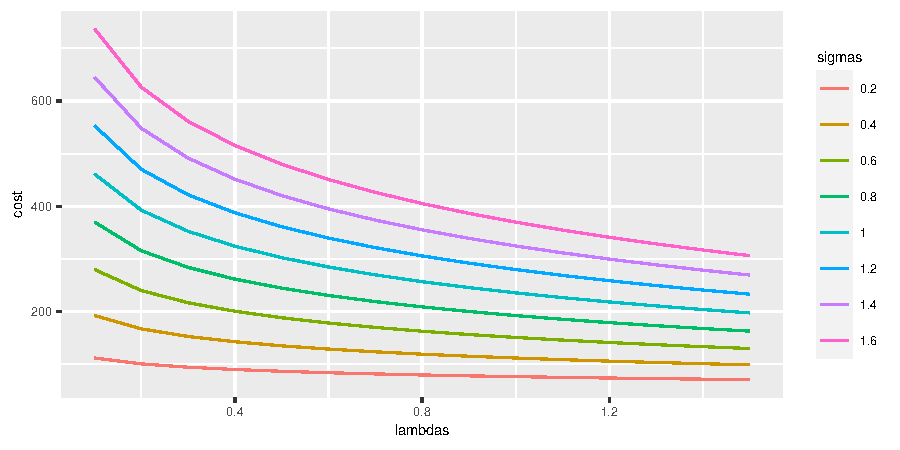
\includegraphics{figs/Chap4/only_cens.pdf}
    \caption{Plot of the cost function values against $\theta$ values when all observations are censored. It is represented for an exponential distribution. The sample consists in 100 values of censored observations to a threshold $a = 0.05$.}
    \label{fig:onlycens}
\end{figure}

We show in the next part why it could be problematic to have fully censored segments in the search method and how we chose to deal with it. 

\subsection{On the detection point method}

The case of fully censored segment are questionning the identifiability of the change-point detection method. The usual assumption \citep{Lavielle1997} for the segment parameters is the following:   
\begin{itemize}
\item[\textbf{H1:}] $\Theta$ is compact and there exists $\Delta_{\bm \theta}^{\star}>0$ such that $\vert \theta_{k+1}^{\star}-\theta_{k}^{\star}\vert > \Delta_{\bm \theta}^{\star}$, for all $k=0,...,K^{\star}$. 
\end{itemize}

We have seen in \ref{chp:4:costex} that, for the exponential distribution example, the optimal $\theta$ tends to infinity. If that is the case $\Theta$ is not compact. To solve this problem, we impose an upper bound $\theta_{max}$ on the possible values of $\theta$. Thus, we have that $\theta \in [0,\theta_{max}]$ which is a compact part of $\mathbbm{R}$. 

A new problem arises from this modeling choice. The value of $\theta_{max}$ must be chosen carefully. We must ensure that $\theta_{max}> \theta^*_k,$ for all $k \in \{0,\dots,K^*\}$. If it is not the case, the identification problem remains. For two $\theta^*_i$ and $\theta^*_j$    greater than $\theta_{max}$, their estimates will be set to $\theta_{max}$ and thus no segment identification will be possible. In order to avoid such problems, the value of $\theta_{max}$ is set according to the worst censoring case scenario possible. More precisely, we assume no change-point occured in $\bm y$ and that all observations are distributed according to $Q$ with parameter $\theta_{max}$. We set $\theta_{max}$ to the value such that: 
$$F(\min(\bm y),\theta_{max})^n = \alpha,$$
with $\alpha$ being a desired percentage of censorship. 

We provide a practical example with the exponential distribution. We simulate a signal $\bm y$ of size $n = 200$ that is a realization of exponential distributions of parameters $\theta^*_0 = 1$ for $y_{1:100}$ and $\theta^*_1 = 4$ for $y_{101:200}$. The censoring level is set to the median of $\bm y$ so that 50$\%$ of the signal is censored. We illustrates $\bm y$ in Figure \ref{fig:theta_max}. We set $\theta_{max}$ choosing with $\alpha = 95\%$. We have that $\theta_{max} = \frac{-\log(1-\alpha^{1/n})}{\min(\bm y)}$. In our numerical example, $\theta_{max} = 24.68$, which is greater than $\theta_0$ and $\theta_1$.

\begin{figure}[ht]
    \centering
    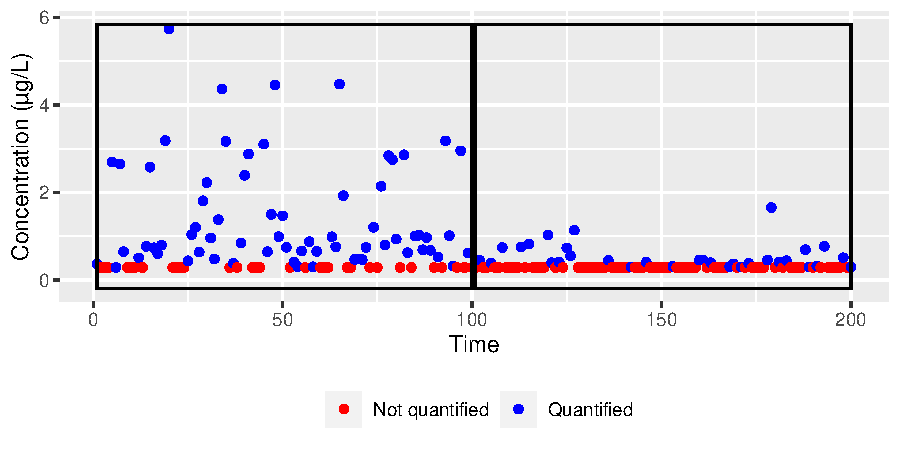
\includegraphics{figs/Chap4/theta_max_ex.pdf}
    \caption{Example of simulated signal $\bm y$ distributed according exponential distributions. The two segments are drawned with black rectangles. $\theta^*_0 = 1$ in the left segment, $\theta^*_1 = 4$ in the right one and the censoring threshold $a = 0.28$ in both segments}
    \label{fig:theta_max}
\end{figure}

Censoring in the data creates identification problems that we chose to deal by adding a new regularisation parameter $\theta_{max}$. Note that other ways to tackle this problem are possible. The modification of the pruning rule \ref{chp:3:pruning} used in PELT can also be investigated. For example, one could decide to systematically discard all potential change-point indices $\tau \in \{u,\dots,v\}$ when evaluating a fully censored segment $y_{u:v}$.  

\section{Multi-dimensional parameter estimation}\label{chp:4:3}

We discuss here the procedure for the parameters estimates proposed in \ref{chp:4:estim}. When $\theta^* \in \mathbb{R}^P$ with $P > 1$, several optimization strategies are possible. We use the following notations in this section: 
\begin{itemize}
\item $\bm \theta_{.,m} = (\theta_{0,m},\dots,\theta_{K,m})$ is the m-th dimension of the parameters vector of each segment $k$.
\item $\bm \theta_{k,.} = (\theta_{k,1},\dots,\theta_{k,P})$ is the parameters vector of the k-th segment.
\item $\theta_{k,m}$ is the m-th dimension of the parameters vector of the k-th segment.
\end{itemize}

A common strategy is to opt for simultaneous changes detection in all $P$ parameters simultaneously. This implies detecting changes in different properties of $\bm y$. An example with $Q$ set as a Weibull distribution is provided in Figure \ref{fig:param_ex}. In practice, it depends on what parameters are optimized in the cost function. The optimization can be petformed with numerical methods (such as Newton-Raphson) on all dimensions of $\theta$ simultaneously. For the k-th segment, let $\widehat{\theta}_{NR} = (\widehat{\theta}_{k,1},\dots,\widehat{\theta}_{k,P})$ the estimates of $\theta_{k,.}$ obtained with Newton-Raphson. Using $\widehat{\theta}_{NR}$ as the supremum in \ref{chp:4:costfunc} provide a cost function that detects changes occuring in any of the parameters.  

\begin{figure}[ht]
    \centering
    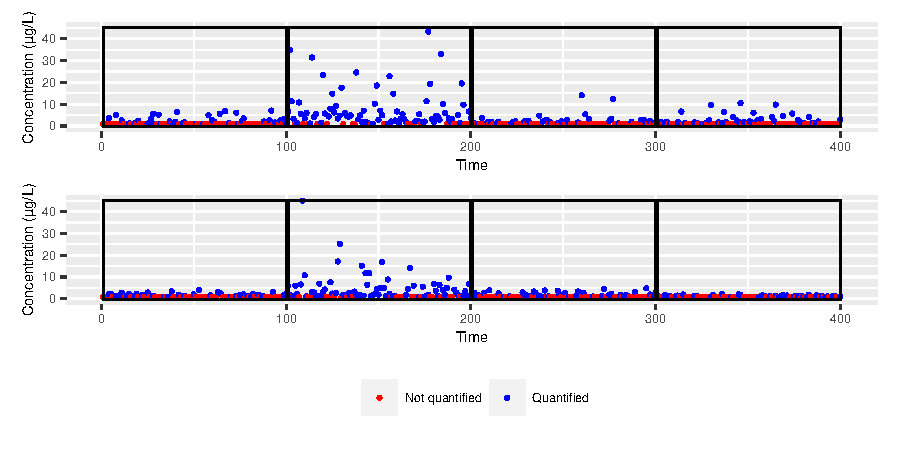
\includegraphics{figs/Chap4/param_ex.pdf}
    \caption{Example of simulated signal $\bm y$ distributed according Weibull distributions with $(\lambda,\sigma)$ as the scale and shape parameters. The segments are drawned with black rectangles. \\ 
\textbf{Upper signal:} The associated parameters to each segment are $\theta^*_{0,.} = (\lambda^*_0,\sigma^*_0) = (1,1)$, $\theta^*_{1,.} = (\lambda^*_1,\sigma^*_1) = (3,0.7)$, $\theta^*_{2,.} = (\lambda^*_2,\sigma^*_2) = (1,0.7)$, $\theta^*_{3,.} = (\lambda^*_3,\sigma^*_3) = (1,2)$ and the censoring threshold $a = 0.86$ in all segments.\\
\textbf{Lower signal:} The associated parameters to each segment are $\theta^*_{0,.} = (\lambda^*_0,\sigma^*) = (1,0.7)$, $\theta^*_{1,.} = (\lambda^*_1,\sigma^*) = (5,0.7)$, $\theta^*_{2,.} = (\lambda^*_2,\sigma^*) = (0.7,0.7)$, $\theta^*_{3,.} = (\lambda^*_3,\sigma^*) = (1,0.7)$ and the censoring threshold $a = 0.89$ in all segments.}
    \label{fig:param_ex}
\end{figure}

We propose a different estimation strategy. We are interested in models where changes occur only in some dimension $\bm\theta^*_{.,m}$. We denote $\mathcal{M} \subset \{1,\dots,P\}$ the set of indices of dimensions where the changes occur and $\overline{\mathcal{M}}$ the complementary set. Figure \ref{fig:param_ex} provides an illustration of signal $\bm y$ simulated from these assumptions. The parameters $(\bm\theta^*_{.,m})_{m \in \overline{\mathcal{M}}}$ are supposed to be fixed throughout the signal $\bm y$. In that setting, the estimation procedure changes. We can rewrite \ref{chp:4:estim} as: 
    
\begin{dmath}\label{chp:4:estimproc}
(\widehat{\TT},\widehat{\theta}_{.,m\in\mathcal{M}},\widehat{\theta}_{.,m\in\overline{\mathcal{M}}}) = \arg\min_{\TT,\bm \theta_{.,m\in\mathcal{M}}}\bigg[\arg\min_{\theta_{.,m\in\overline{\mathcal{M}}}}\bigg\{ - \sum_{i=0}^{\lvert \TT \rvert}  \left(\sum_{j=\tau_i+1}^{\tau_{i+1}}\log(F(y_j,\theta))\mathbbm{1}_{y_j=a_j}+\sum_{j=\tau_i+1}^{\tau_{i+1}}\log(f(y_j,\theta))\mathbbm{1}_{y_j>a_j}\right)\bigg\}+\beta KP \bigg]
\end{dmath}

From \ref{chp:4:estimproc}, we can design a two-step iterative estimation strategy. The two steps of each iteration are:
\begin{enumerate}
\item Compute the MLE $\widehat{\bm\theta}_{{.,m\in\overline{\mathcal{M}}}}$ with fixed $\widehat{\TT}$ and $\widehat{\theta}_{.,m\in\mathcal{M}}$ with any optimization method that handles censored data. We use \texttt{R} package developped in \cite{delignette2015} in our procedure.  
\item Run the change-point procedure to estimate $\widehat{\TT}$ and $\widehat{\theta}_{.,m\in\mathcal{M}}$ using the values of $\widehat{\bm\theta}_{{.,m\in\overline{\mathcal{M}}}}$.
\end{enumerate} 

In the second step of the iteration, the estimated segmentation $\widehat{\TT}$ and the fitted parameters on its segments $\widehat{\theta}_{.,m\in\mathcal{M}}$ are obtained by applying the PELT procedure \citep{Killick2012}. PELT is run several times on a penalty grid $(\beta_0,\dots,\beta_q,\dots,\beta_{B})$ where $\beta_0<\dots<\beta_{q}<\dots<\beta_{B}$ are evenly spaced. We obtain $B$ segmentations of $\bm{y}$. Eventually, the optimal penalty value for this step is selected using an elbow rule heuristic as proposed in Section \ref{chp:3:2}.

The initialization is an important part of this procedure. We would like the initial estimate of the fixed parameters to be close to $\bm\theta^*_{{.,m\in\overline{\mathcal{M}}}}$ to ensure the convergence of the procedure. In order to do so, we intialise $\widehat{\bm\theta}$ assuming no change-point occured in $\bm y$.  More formally, we compute: 
\begin{equation}\label{chp:4:init}
\widehat{\bm\theta} = \arg\min_{\theta}\bigg\{ - \left(\sum_{j=1}^{n}\log(F(y_j,\theta))\mathbbm{1}_{y_j=a_j}+\sum_{j=1}^{n}\log(f(y_j,\theta))\mathbbm{1}_{y_j>a_j}\right)\bigg\}
\end{equation}   
We proceed using the MLE estimator for all parameters in $\bm \theta$, which implies using iterative methods again as stated in \cite{cohen1965maximum}. We choose the initial values as the $\widehat{\bm\theta}_{.,m}$ such that $m\in\overline{\mathcal{M}}$. It can be noted straight away that the value of $\widehat{\bm\theta}_{.,m\in\mathcal{M}}$ will be discarded since it was computed from a model that goes in direct contradiction with the assumption in \ref{chp:4:1} that they were change-points in the signal $\bm y$. We show the efficiency of this procedure in Appendix \ref{app:chap4:3}.  

We use this procedure estimation in Chapter \ref{chp:5}. We justify this choice with the observation of real data. We compare the efficiency of our method a state-of-the-art in the next section.

\section{Simulation study}\label{chp:4:4}

We test our method on simulated data and compare it with the \textit{Multrank} method \cite{lung2015}. This section aims at two objectives. First, we want to calibrate the parameters of our method to ensure good efficiency. Then, we want to test if that calibration really leads to better change-point results.  

\subsection{Calibration of the minimal segment length}

In section \ref{chp:2:2}, the PELT Algorithm \ref{chp:3:algopelt} introduces a minimal segment length $n_{min}$. We lead some simulation tests to calibrate its value. We need to identify $n_{min}$ so that the cost function defined in \ref{chp:4:costfunc} has sufficient data to make the difference between segments on which the parameters differ. 

This task can be viewed as a classification one. We want to know if our method is able to classify correctly signals that have a change point or not. Since we use a parametric inference (see Section \ref{chp:4:1}), we use the log likelihood ratio test to assess the presence of a change-point. This is a very common test used in change-point that can be found in. The statistics of the likelihood ratio test are calculated on several simulated signals and and the ROC curves \citep{Fawcett2006} are derived from it. We compute the corresponding areas under the curve (AUC) to assess the ability to detect change-points of our method. A comparison of our method is made with the \textit{MultRank} method that is based on non parametric inference that we presented in Section \ref{chp:3:1}. We will use this comparison to calibrate our method performance.  

The simulation procedure for the calibration of $n_{min}$ is the following. We use the Weibull distribution for the distribution $Q$. We test several configurations with different censoring levels $\alpha = (5\%,25\%,50\%,75\%,95\%)$. It is a global censoring level, meaning that for a given signal $\bm y$, $\alpha\%$ of the data is censored. The detection methods are run with different values of minimal segment size $n_{min} = (5,10,25,50,75)$. For each configuration, we simulate $M = 1000$ signals of size $n = 200$ among which half of them present a change point in position 100. The parameters of signals with a change-point are $(\sigma = 0.5,\lambda^*_0 = 1)$ on the first segment and $(\sigma = 0.5,\lambda^*_1 = 3)$ on the second. The parameters associated to signals with no change-point are $(\sigma = 0.5,\lambda = 1)$. We compute the AUC on these $M$ signals. The results are illustrated in Figure \ref{fig:sim_minseg}.      

\begin{figure}[ht]
\centering
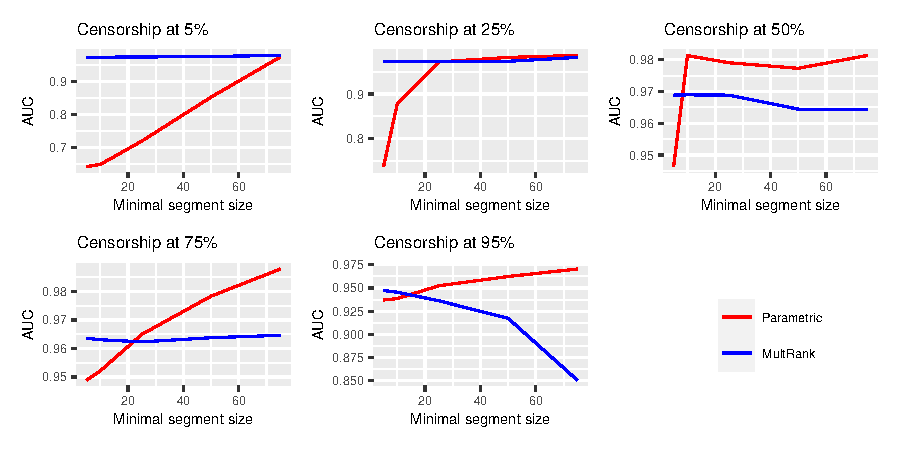
\includegraphics{figs/Chap4/sim_minseg.pdf}
\caption{Choice of the minimal segment length: simulation results. Our method performance is Illustrated with the red dots, the \textit{Multrank} method is drawn in blue.}
\label{fig:sim_minseg}
\end{figure}

From the results of Figure \ref{fig:sim_minseg}, three comments can be made:  
\begin{itemize}
\item Both methods are efficient in their abilities to detect change-points in signal. The AUC are above 0.9 (except for the parametric method in a highly censored configuration with a low value minimal segment size). That make them both good classifiers. 
\item The performance of the parametric method increases with the minimum segment length. 
\item The more the censoring levels increase, the more data is needed in the minimal segment length of the parametric method to outclass the non parametric method. 
\end{itemize}
From this study, we can conclude that when working with real data, we should get the censoring level information information in order to calibrate the minimal segment length of the parametric method.  

\subsection{Comparison with a non parametric method}

We want to compare the performance of the change-point detection with the Multrank method developped in \cite{lung2015} since both methods are adapted to censored data. We examine the capacity to estimate the correct number of breaks in a signal and the precision of the change-point position. This section is illustrated using the Weibull distribution.   

The experimental framework is as follows: 
    \begin{enumerate}
        \item we simulate $N=100$ samples $(x_1,...,x_n)$ of size $n=400$  following a left-censored Weibull distribution with $\alpha\%$ of censored data. We made tests for the different censorship rates $\alpha = (25,50,75,95)$. The shape parameter of the Weibull distribution is assumed to be known and set to $\sigma=0.5$. The scaling parameters $\bm{\lambda^\star}$ have $K^\star=4$ breaks at positions $p^\star_1 = 80$, $p^\star_2 = 160$, $p^\star_3 = 240$ and $p^\star_4 = 320$ and take the values $\bm{\lambda^\star}=(\lambda^\star_1 = 1, \lambda^\star_2 = 4, \lambda^\star_3 = 0.5, \lambda^\star_4 = 5, \lambda^\star_5 = 1)$. An example of a sample simulated in this way is shown in Figure \ref{fig:ex_sim}.
        \item For each of the $N$ samples, we perform the parametric change-point detection and the Multrank methods. For each sample, we obtain the estimated number of breaks $\hat K_{param}$ and $\hat K_{multrank}$ and their position $(\hat{p}_{k,param})_{k = 1}^{\hat K_{param}}$ (respectively $(\hat{p}_{k,multrank})_{k = 1}^{\hat K_{multrank}}$).
        \item for both methods, we count the number of samples among the $N$ for which the correct number of breaks has been estimated (e.g. $\hat K_{param} = K^\star$). Also, for each of the samples for which the estimate of $K^\star$ is correct, we make an histogram of the change-points position. 
    \end{enumerate}
Since $K$ is not known, we proceed as follows for each method to estimate it:
    \begin{itemize}
        \item For the parametric method: we use the algorithm CROPS, algorithm to scan a continuous range of penalty values $[\beta_{min},\beta_{max}]$. We obtain a set of $B$ values $(\hat \beta_1,...,\beta_B)$ and the optimal segmentations associated with these penalty values. We then plot the cost of the segmentations as a function of the number of breaks. We choose the optimal penalty using a elbow heuristic. This procedure is described in \cite{haynes2014}. The choice of $\beta_{min}$ and $\beta_{max}$ is inspired from linear penalties like the BIC criterion \cite{YAO1988181}. Note that when using the BIC penalty in change point detection, the penalty term written in section \ref{chp:4:1} becomes : $\beta_n = \frac{P}{2}\log(n) = \frac{1}{2}\log(n)$, where $P$ is the number of dimensions of the parameter. More precisely, we took a wide interval of penalty values defined by $\beta_{min} = \frac{\log(n)}{10}$ and $\beta_{max} = 5\log(n)$.
        \item For the non parametric \textit{Multrank} method, we compute using the optimal segmentation search method presented in Algorithm \ref{chp:3:algoopt} for $k$ breaks, where $k$ ranges from $1$ to $K_{max}$. For each of these segmentations, we can compute the cost of the segmentations using the cost function explicited in \ref{chp2:costfuncnp}. As in the parametric method, we represent the costs as a function of $k$, and we determine the number of estimated breaks by an elbow heuristic. Here, $K_{max}$ is fixed at $2*K^\star = 8$.
    \end{itemize}
The results of the simulations are shown in Table \ref{tab:simcomp} and in Figure \ref{fig:prec_sim}. It can be seen that in the ideal scenario, where the data are indeed distributed according to a left-censored Weibull distribution, the parametric method performs better both in detecting the correct number of breaks and in accurately estimating their position. However, this performance decreases as the censoring rate increases.

\begin{figure}[ht]
    \centering
    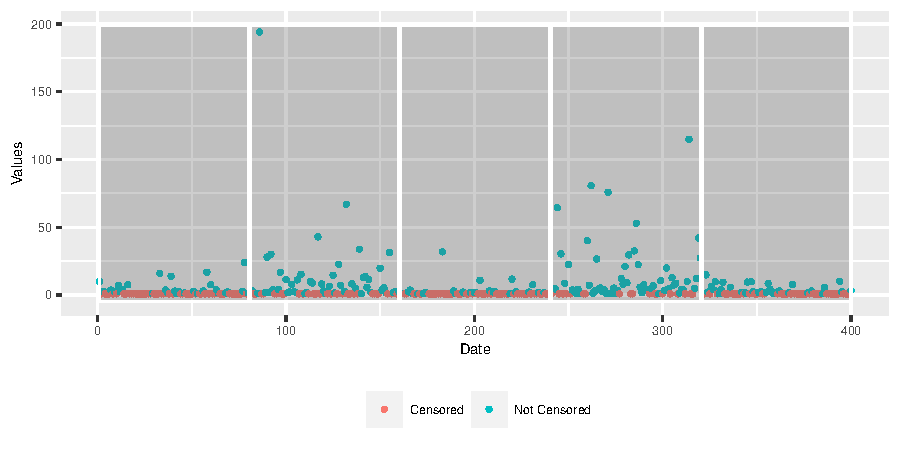
\includegraphics{figs/Chap4/Ex_sim.pdf}
    \caption{Example of simulated signal with $(\lambda_1 = 1, \lambda_2 = 4, \lambda_3 = 0.5, \lambda_4 = 5, \lambda_5 = 1)$, $\sigma = 0.5 $, $n = 400$, $K = 4$, $(p_1 = 80,p_2 = 160,p_3 = 240,p_4 = 320)$ and $\alpha = 50\%$.}
    \label{fig:ex_sim}
\end{figure}

\begin{table}[ht]
\centering
\begin{tabular}{|r|r|r|}
  \hline
   $\alpha(\%)$  & Parametric method & MultRank \\ 
  \hline
 25 &  84 &  58 \\ 
 50 &  80 &  63 \\ 
 75 &  87 &  68 \\ 
 95 &  65 &  10 \\ 
   \hline
\end{tabular}
\caption{Number of correct estimations of $K$ over $N=100$ samples for both methods for different $\alpha\%$ censorship rates.}
\label{tab:simcomp}
\end{table}

\begin{figure}[ht]
    \centering
    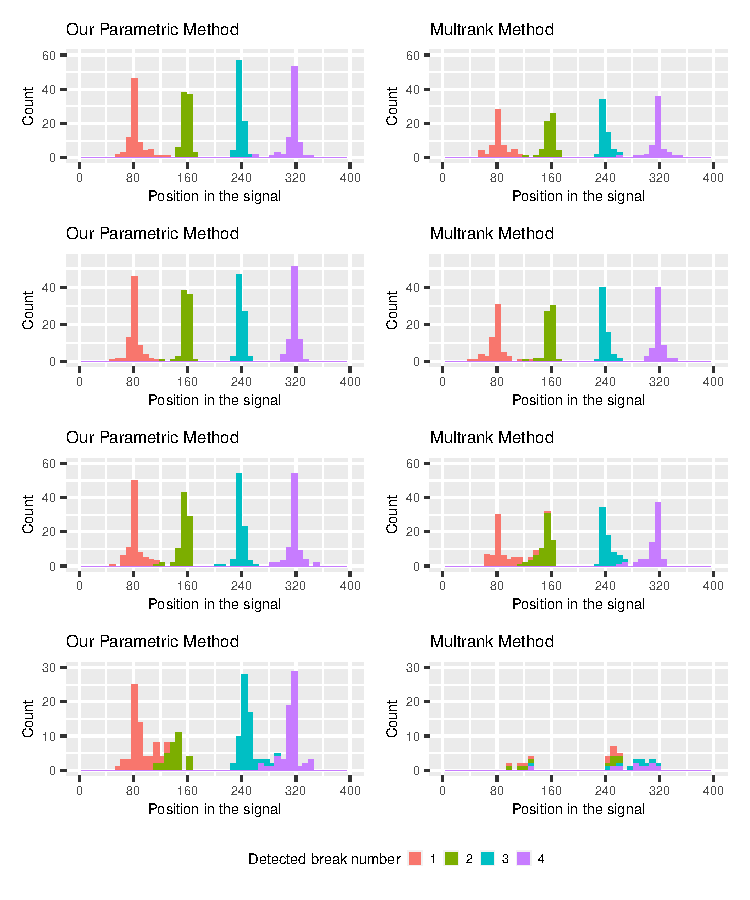
\includegraphics{figs/Chap4/detect_comp.pdf}
    \caption{Precision of the estimated change-points for both methods.}
    \label{fig:prec_sim}
\end{figure}

\clearpage

\section{Chapter summary}

This Chapter designs and tests an adapted method for change-point detection for concentration data. The censorship is dealt with the cost function choice in Section \ref{chp:4:2}. More precisely, using a parametric approach as presented in Chapter \ref{chp:3}, the likelihood is adapted to distinguish cases were a measure is censored or not. The censorship becomes critical for computing the maximum likelihood estimate of a segment when all observations are censored. This could cause issues in the identification of segments parameters which would compromise the detection method capacity. However, one way to circumvent this problem is to indroduce a new regularization parameter in the detection that is a maximum value for the parameter value. The estimation strategy is also discussed in this Section \ref{chp:4:3}. An esitmation scheme where some parameters dimension are fixed in time and other can vary accross segments is devised. In practice, this modeling choice can be justified if some parameters values are supposed to control the intrinsic diffusion properties of a chemical substance in the environment. Then, these parameters should be invariant in time. The parameters changing at each segment could represent the different use intensity of the substance in time for example. Experiments of Section \ref{chp:4:4} ensures that, if enough data is availbale to evaluate a segment, the parametric method fares decently and can outclass a suited non parametric method for censored data. 

Chapter \ref{chp:5} combines the results of temporal change-point detection using the parametric method developped in this Chapter with statistical methods to deal with the spatial heterogeneity. The obtention of homogenous temporal subsignal in the concentrations values provides the temporal context in which the spatial analysis is conducted. In particuliar, in this homogenous temporal setting, it is interesting to look for geographical areas that had concentration values that differ from others. Constructing these areas and comparing them is the main topic of Chapter \ref{chp:5}. Chapter \ref{chp:6} is the presentation of the results of Chapter \ref{chp:5} and \ref{chp:4} applied to the concentration data of substance. The results of all methods are all gathered using an interactive presentation tool.     

       

 